\section{Background}
In this section we describe MAPF and ASP. Our definition of MAPF follows closely that of \acite{SternSFK0WLA0KB19}. 

\subsection{Multi-Agent Pathfinding}
A MAPF instance is defined by a tuple $(G,\mathcal{A},init,goal)$, where $G=(V,E)$ is a graph, $A$ is the set of agents, and $init:A\rightarrow V$ and $goal:A\rightarrow V$ are functions used to denote the initial and goal vertex for each of the agents.

At each time instant each agent at vertex $v$ can either move to any of its successors in $G$ or not move at all. When the graph $G$ is a 4-connected grid, as we assume in the rest of the paper, there are 5 possible moves at each time instant: $\{\Up,\Down,\Left,\Right,\Wait\}$, where the first four move the agent in one of the four cardinal positions, and the \Wait move results in the agent staying at its current vertex. A \emph{path} over $G$ is a sequence of vertices in  $V$, $v_1v_2\ldots v_n$, where either $v_i=v_{i+1}$ (i.e., a \Wait action is performed) or $(v_i,v_{i+1})\in E$ (i.e., a non wait action is performed) for every $i\in\{1,\ldots,n-1\}$. Given a path $\pi$ we denote by $\pi[i]$ the $i$-th element in $\pi$, where $i\in\{1,\ldots,|\pi|\}$.

A solution to MAPF is a function $sol:\mathcal{A}\rightarrow V^*$, which associates a path to each of the agents, such that the first and last vertices of $sol(a)$ are, respectively, $init(a)$ and $goal(a)$. Without loss of generality henceforth we assume that all paths in $sol$ have the same size, since wait actions may be used at the end of any action sequence to remain on the same vertex. Below we denote by $\mathcal{T}$ the set $\{1,\ldots,M\}$, where $M$ is the size of any of the paths in $sols$. We also refer to $M-1$ as the \emph{makespan} of the solution.

In addition, $sol$ must be \emph{conflict-free}, which means that if $\pi$ and $\rho$ are the paths in $sol$ followed by two different agents, none of the following conflicts should arise.
\begin{itemize}
    \item \textbf{Vertex Conflict}. Two agents cannot be at the same vertex at the same time instant. Formally, there is a vertex conflict iff $\pi[i]=\rho[i]$, for some $i\in\mathcal{T}$.
    \item \textbf{Swap Conflict}. Two agents cannot swap their positions. Intuitively, this conflict is justified by that fact that we assume that size of the agents prevent the connection between two vertices in opposite directions. Formally, there is a swap conflict iff $(\pi[i],\rho[i])=(\rho[i+1],\pi[i+1])$, for some $i\in\{1,\ldots,M-1\}$.
\end{itemize}
Following most of the literature in MAPF (e.g., \nbcite{SharonSFS12}), we consider only these two types of conflicts, and no other conflicts. For example, we do not consider so-called \emph{following conflicts} \cite{SternSFK0WLA0KB19}, which do not allow an agent to occupy at time $t+1$ the position of another agent had at time $t$.

A standard assumption in MAPF is that all actions cost one cost unit unless wait actions that are performed by agents at the goal when no other action is planned in the future. Thus the cost of path $\pi$ for agent $a$ is written as $|\rho|$, when $\rho$ is the shortest sequence such that $\pi=\rho(goal(a))^k$, for some $k$. The cost of a solution $sol$ is defined as $\sum_{a\in A} c(sol(a))$.

A solution $sol$ is \emph{optimal under sum-of-costs}, or simply \emph{cost-optimal}, if no other solution $sol'$ exists such that $c(sol')<c(sol)$. A solution $sol$ is makespan-optimal, if no other solution exists whose makespan is smaller than the makespan of $sol$. A makespan-optimal solution is not necessarily a cost-optimal solution. This is illustrated in Figure ~\ref{fig:makespancost}.

\begin{figure}
    \centering
    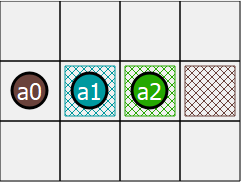
\includegraphics[width=0.24\textwidth]{graphs/makespangrid.PNG}
      \caption{Problem instance where the increase of makespan yields better \emph{sum-of-costs} solutions. The problem has 3 agents:  $a_0$, who needs to go from $(0,1)$ to $(3,1)$. And agents $a_1$ and $a_2$ who are already at the goal at the positions $(1,1)$ and $(2,1)$ respectively. The optimal cost solution with makespan $3$ is $8$ as it involves $a_1$ and $a_2$ moving away from their goal to make space for $a_0$. In contrast the optimal cost solution with makespan $5$ is $5$ as it only needs to move $a_0$.}
    \label{makespancost}
\end{figure}


\subsection{Answer-Set Programming}
ASP \cite{Lifschitz08} is a logic-based framework for solving optimization problems. For space limitations, here we describe a subset of an ASP standard that is relevant to this paper.

An ASP \emph{basic program} is a set of rules of the form:
\begin{equation}\label{asprule}
p\leftarrow q_1,q_2,\ldots,q_n
\end{equation}
where $n\geq 0$, and $p$, $q_1,\ldots,q_n$ are so-called \emph{atoms}. The intuitive interpretation of this rule is as follows ``p is true/provable if so are $q_1,q_2,\ldots,q_n$''. When $n=0$ rule \eqref{asprule} is considered to have an empty body. Such rules are called facts and are usually written as `$p$' instead of `$p\leftarrow $'.

A \emph{model} of an ASP basic program is a set of atoms $M$ that intuitively contains all and only the atoms that are provable. Formally, $M$ is a model of basic program $\Pi$ iff $M$ is the subset-minimal set such that for every rule $p\leftarrow q_1,q_2,\ldots,q_n \in \Pi$ such that $\{q_1,\ldots,q_n\}\subseteq M$, then $p\in M$.



An important syntactic element relevant to our paper is the so-called \emph{negation as failure}. Rules containing such negated atoms look like:
\begin{equation}\label{negasprule}
p\leftarrow q_1,q_2,\ldots,q_n, not\: r_1,not\: r_2, \ldots, not\: r_k .
\end{equation}
Intuitively, rule \eqref{negasprule} should be interpreted as `$p$ is provable if $q_1,\ldots q_n$ are provable a none of $r_1,\ldots,r_k$ are provable'. The semantics of programs that include negation as failure is simple but a little more involved, require the introduction of so-called \emph{stable models}, whose formal definition we omit from this paper. We direct the interested reader to the paper by \acite{FerrarisL05}.

%e a of set of ntatoms $M$ is a model of a program $P$ containing such rules if the \emph{reduct} of $\Pi$ with respect to $M$, denoted as $\Pi^M$ also has $M$ as a model. Intuitively $P^M$ is a basic program which results from simplifying away every occurrence of a $not\:p$ in the obvious way (i.e., eliminating the rule if $p$ is in the model $M$, and removing $not\:p$ from the rule if $p$ is not in the model $M$). For example $M=\{p\}$ is a model of $\Pi=\{p\leftarrow not\: q\}$, since $\Pi^M=\{p\leftarrow \}$ has $M$ as a model. $M'=\{q\}$ is not a model of $\Pi$ since $\Pi^{M'}=\{\}$ does not have $M'$ as a model.

Another relevant type of rule for our paper is:
\begin{equation*}
    |\{p_1,p_2,\ldots,p_n\}|=k \leftarrow q_1,q_2,\ldots,q_n.
\end{equation*}
Intuitively here we say that if $q_1,q_2,\ldots,q_n$ are all provable, then $k$ of the elements in $\{p_1,p_2,\ldots,p_n\}$ must appear in the model. This definition allows programs to have multiple models\footnote{Technically, negation as failure alone also allows the user to create programs with multiple models, but in our translation we define multiple models exploiting this type of rule.}. For example, the program:
\begin{align*}
    &s\\
    &|{p,q,r}|=1\leftarrow s
\end{align*}
has three models: $\{p,s\}$, $\{q,s\}$, and $\{r,s\}$.

Another type of rule that is relevant to our translation is:
\begin{equation}
    \leftarrow p_1,p_2,\ldots,p_n
\end{equation}
which is a constraint that prohibits the occurrence of $\{p_1,p_2,\ldots,p_n\}$ in the model.

Finally, ASP programs may contain variables to represent rule \emph{schemas}. As such, a rule like:
\begin{equation}\label{aspwithvariables}
    p(X)\leftarrow q(X)
\end{equation}
where uppercase letters represent \emph{variables}. Intuitively a variable can take any value among the set of \emph{terms}. As such, rule \eqref{aspwithvariables} represents that when $c$ is a term and $q(c)$ is provable, so is $p(c)$. Intuitively a term represents an object that can be named in the program. The set of terms for a program is syntactically determined from the program using the constants mentioned in it. The set of terms has a theoretical counterpart, the so-called \emph{Herbrand base}, whose definition we omit here, since it is not key for understanding the rest of the paper.

What is key to understand for the rest of the paper, because it affects our conclusions, is that in the process of finding a model for a program an initial step that is carried out is \emph{grounding}, which removes variables from the program. Since there are plenty of optimizations that can be carried out during grounding time it is not easy to describe the grounding process with complete precision. For example, the grounded version for program
\begin{equation}
    \{q(a),q(b),p(X)\leftarrow q(X)\}
\end{equation} may be
\begin{align*}
&\{q(a),q(b),p(a)\leftarrow q(a),p(b)\leftarrow q(b)\} \text{ or } \\
&\{q(a),q(b),p(a),p(b)\},
\end{align*}
depending on the optimizations applied at grounding time. What is however unavoidable is that grounding generates two instances for the rule $p(X)\leftarrow q(X)$ because the number of objects that satisfy predicate $q$ is two. Thus if we had declared $n$ objects satisfying $q$ we would expect the grounding process to generate $n$ instances for $p(X)\leftarrow q(X)$. As we will see in the rest of the paper, the size of the grounded version of the program is key for performance.
